Die im Folgenden beschriebene Methodik zur Bestimmung der deflektometrischen Registrierung ist ein mehrstufiges Phasenschiebeverfahren.
Ein solches Verfahren wird von Kammel in seiner Dissertation \cite{kit_kammel} vorgestellt.
Das Verfahren von Kammel zeigt jedoch in der Praxis Kodierungsartefakte bzw. Phasensprünge insbesondere an den Periodengrenzen.
Aus dem Grund stellt Werling darauf aufbauend in seiner Dissertation \cite{kit_werling} einen neuen Ansatz eines mehrstufigen Phasenschiebeverfahrens vor, der das Problem mit den Phasensprüngen minimiert.
Die Idee des Ansatzes ist dabei, dass man zunächst analog zum Verfahren aus dem vorigen Abschnitt \ref{sub:registrierungOhnePhasenentfaltung} die $x$- bzw. $y$-Koordinaten relativ zu den Perioden der Muster bestimmt.
Durch mehrere Muster mit unterschiedlichen Perioden erhält man schließlich unterschiedliche relative $x$- bzw. $y$-Koordinaten.
Diese müssen für das finale Ergebnis jeweils den richtigen Perioden zugeordnet werden, indem ein Gleichungssystem aufgestellt wird.

\p
Analog zum Verfahren aus Kapitel \ref{sub:registrierungOhnePhasenentfaltung} benötigt man $N_{shift}$-viele phasenverschobene Muster, um die Phase eines Bildpunkts $(x_B, y_B)^\top$ zu bestimmen.
Zusätzlich betrachtet man mehrere Stufen des Verfahrens.
Die Muster auf der Stufe $i$ haben $N_p^i$-viele Perioden über die Monitorbreite \acrshort{lwidth} bzw. Monitorhöhe \acrshort{lheight}.
Auf unterschiedlichen Stufen des Verfahrens sollen stets auch die Anzahlen der Perioden der Muster unterschiedlich sein.
Auf jeder Stufe des Verfahrens befinden sich $N_{shift}$-viele phasenverschobene Muster, welche dieselbe Anzahl an Perioden $N_p^i$ entlang der Monitorbreite bzw. Monitorhöhe haben.
Das heißt, dass die Muster auf der $i$-ten Stufe identisch sind, bis auf die Phasenverschiebung.
Die Phasen $\phi_x^i$ und $\phi_y^i$ der kodierten Monitorpunkte $(x_L, y_L)^\top$ auf der $i$-ten Stufe sehen dann folgendermaßen aus:
%
\begin{equation}
	\phi_x^i = \dfrac{2\pi N_p^i}{\acrshortmath{lwidth}} x_L,
	\qquad
	\phi_y^i = \dfrac{2\pi N_p^i}{\acrshortmath{lheight}} y_L
\end{equation}

\p
O.B.d.A. wird unter Verwendung von Satz \ref{theo:separierbarkeitDeflektometrischeRegistrierung} nachfolgend nur die deflektometrische Registrierung der Spaltenpositionen \acrshort{lrx} ($x$-Richtung) betrachtet.
Die deflektometrische Registrierung der Zeilenpositionen \acrshort{lry} ($y$-Richtung) kann analog bestimmt werden.
Auf der Stufe $i$ hat das $k$-te Muster $m_k^i$ zur Kodierung der Monitorpunkte $(x_L, y_L)^\top$ somit die Form:
%
\begin{equation}\label{eq:monitormuster_mehrstufig}
	\begin{gathered}	
		m_k^i(x_L,y_L) = A_m^i \left(1 + C_m^i \cos \left(\phi_x^i + \psi_k\right)\right),\\
		k \in \lbrace 1,\ldots,N_{shift}\rbrace,
		\quad
		\psi_k = (k - 1)\dfrac{2\pi}{N_{shift}}
	\end{gathered}
\end{equation}
%
$A_m^i$ bezeichnet die Amplitude und $C_m^i$ den Kontrast der Muster der $i$-ten Stufe.
Wie auch in Abschnitt \ref{sub:registrierungOhnePhasenentfaltung} entspricht $\psi_k$ der Phasenverschiebung des $k$-ten Musters und $N_{shift}$ der Anzahl der Phasenverschiebungen.
Der Einfluss der jeweiligen Parameter ist analog zu Abschnitt \ref{sub:registrierungOhnePhasenentfaltung} und einsehbar in Abbildung \ref{tikz:abbBeispielMusterOhnePhasenentfaltung}.
Abbildung \ref{tikz:abbBeispielMusterMitPhasenentfaltung} zeigt eine mögliche Musterserie für dieses Verfahren, um das Verständnis zwischen den Mustern und den Stufen aufzuzeigen.
%
% Abbildung: Beispiel Muster
{
	\begin{figure}[H]
		\centering
		\begin{adjustbox}{width=\textwidth}
	\begin{tikzpicture}[every node/.style={inner sep=0,outer sep=0}]
		
		%Bilder Stufe 1
		\node [anchor=north west] (img11) at (0.1\textwidth,0) {
\includegraphics[frame,width=.28\textwidth]{04_deflektometrischeRegistrierung/bestimmungDeflektometrischeRegistrierung/registrierungMitPhasenentfaltung/figures/m_1_1}};
		\node [anchor=north west] (img21) at (0.41\textwidth,0) {
\includegraphics[frame,width=.28\textwidth]{04_deflektometrischeRegistrierung/bestimmungDeflektometrischeRegistrierung/registrierungMitPhasenentfaltung/figures/m_2_1}};
		\node [anchor=north west] (img31) at (0.72\textwidth,0) {
\includegraphics[frame,width=.28\textwidth]{04_deflektometrischeRegistrierung/bestimmungDeflektometrischeRegistrierung/registrierungMitPhasenentfaltung/figures/m_3_1}};
		
		%Bilder Stufe 2
		\node [below=1cm of img11.south west, anchor=north west] (img12) {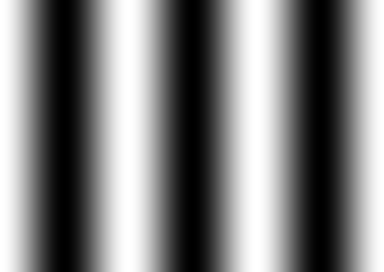
\includegraphics[frame,width=.28\textwidth]{04_deflektometrischeRegistrierung/bestimmungDeflektometrischeRegistrierung/registrierungMitPhasenentfaltung/figures/m_1_2}};
		\node [below=1cm of img21.south west, anchor=north west] (img22) {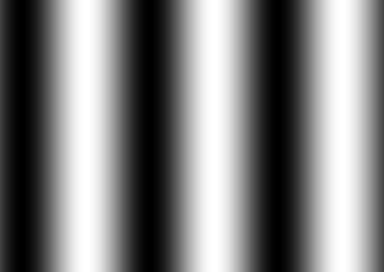
\includegraphics[frame,width=.28\textwidth]{04_deflektometrischeRegistrierung/bestimmungDeflektometrischeRegistrierung/registrierungMitPhasenentfaltung/figures/m_2_2}};
		\node [below=1cm of img31.south west, anchor=north west] (img32) {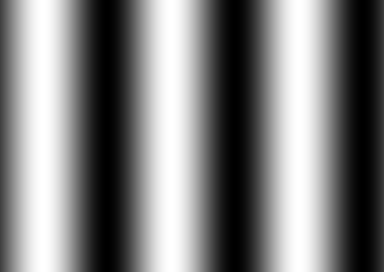
\includegraphics[frame,width=.28\textwidth]{04_deflektometrischeRegistrierung/bestimmungDeflektometrischeRegistrierung/registrierungMitPhasenentfaltung/figures/m_3_2}};
	
		%Bilder Stufe 3
		\node [below=1cm of img12.south west, anchor=north west] (img13) {
\includegraphics[frame,width=.28\textwidth]{04_deflektometrischeRegistrierung/bestimmungDeflektometrischeRegistrierung/registrierungMitPhasenentfaltung/figures/m_1_3}};
		\node [below=1cm of img22.south west, anchor=north west] (img23) {
\includegraphics[frame,width=.28\textwidth]{04_deflektometrischeRegistrierung/bestimmungDeflektometrischeRegistrierung/registrierungMitPhasenentfaltung/figures/m_2_3}};
		\node [below=1cm of img32.south west, anchor=north west] (img33) {
\includegraphics[frame,width=.28\textwidth]{04_deflektometrischeRegistrierung/bestimmungDeflektometrischeRegistrierung/registrierungMitPhasenentfaltung/figures/m_3_3}};
		
		%Captions Stufe 1
		\node [below=0.2cm of img11] (cap11) {Muster $m_1^1$};
		\node [below=0.2cm of img21] (cap21) {Muster $m_2^1$};
		\node [below=0.2cm of img31] (cap31) {Muster $m_3^1$};
		
		%Captions Stufe 2
		\node [below=0.2cm of img12] (cap12) {Muster $m_1^2$};
		\node [below=0.2cm of img22] (cap22) {Muster $m_2^2$};
		\node [below=0.2cm of img32] (cap32) {Muster $m_3^2$};
		
		%Captions Stufe 3
		\node [below=0.2cm of img13] (cap13) {Muster $m_1^3$};
		\node [below=0.2cm of img23] (cap23) {Muster $m_2^3$};
		\node [below=0.2cm of img33] (cap33) {Muster $m_3^3$};
		
		
		%Beschriftung Stufen
		\node [left=0.7cm of img11.west, anchor=east] {Stufe 1:};
		\node [left=0.7cm of img12.west, anchor=east] {Stufe 2:};
		\node [left=0.7cm of img13.west, anchor=east] {Stufe 3:};
		
		%Beschriftungen Phasenverschiebungen
		\node [above=0.2cm of img11] {$k = 1$ $\left(\psi_1 = 0\right)$};
		\node [above=0.2cm of img21] {$k = 2$ $\left(\psi_2 = \tfrac{2\pi}{3}\right)$};
		\node [above=0.2cm of img31] {$k = 3$ $\left(\psi_3 = \tfrac{4\pi}{3}\right)$};
		
	\end{tikzpicture}
\end{adjustbox}
\caption[Muster mit unterschiedlichen Perioden zur Phasenkodierung]{Musterserie nach Gleichung \ref{eq:monitormuster_mehrstufig} mit $A_m =127.5$, $C_m = 1.0$, $N_{shift} = 3$, $\acrshortmath{lwidth} = 384$, Anzahlen an Perioden $N_p^1 = 2$, $N_p^2 = 3$ und $N_p^3 = 5$}
		\label{tikz:abbBeispielMusterMitPhasenentfaltung}
	\end{figure}
}

\noindent
Für jedes Muster jeder Stufe nimmt die Kamera Signale $g_k^i$ auf:
%
\begin{equation}\label{eq:kamerabild_mehrstufig}
	g_k^i(x_B, y_B) = A_g^i(x_B, y_B) \left(1 + C_g^i(x_B, y_B) \cos \left(\dfrac{2\pi N_p^i}{\acrshortmath{lwidth}}\acrshortmath{lrx}(x_B, y_B) + \psi_k\right)\right)
\end{equation}
%
Analog zu Kapitel \ref{sub:registrierungOhnePhasenentfaltung} lässt sich aus den Bildern $g_k^i$ die Phase der $i$-ten Stufe $\phi_x^i$ berechnen.
Vergleichbar mit Gleichung \ref{eq:registrierungX} kann man in diesem Verfahren aus der Phase die Monitorkoordinaten relativ zum Intervall $[0,\acrshortmath{lwidth}/N_p^i)$ bestimmen:
%
\begin{equation}\label{eq:registrierungX_relativ}
	x_{L,relativ}^i =
	\dfrac{\acrshortmath{lwidth}}{2\pi N_p^i}
	\arctan 
	\left( 
		-\dfrac
		{\sum\limits_{k=1}^{N_{shift}} g_k^i(x_B, y_B) sin\left((k - 1)\dfrac{2\pi}{N_{shift}}\right)}
		{\sum\limits_{k=1}^{N_{shift}} g_k^i(x_B, y_B) cos\left((k - 1)\dfrac{2\pi}{N_{shift}}\right)}
	\right)
\end{equation}
%
Die absolute Monitorkoordinate $x_L^i$ der $i$-ten Stufe lässt sich bestimmen, indem man zur Phase $\phi_x^i$ ein unbekanntes ganzzahliges Vielfaches von $2\pi$ addiert.
In Abhängigkeit von $x_{L,relativ}^i$ bedeutet das für $x_L^i$:
%
\begin{equation}\label{eq:registrierungX_absolut}
	x_L^i = x_{L,relativ}^i + n^i \dfrac{\acrshortmath{lwidth}}{N_p^i},
	\qquad
	(n^i \in \mathbb{N}_0)
\end{equation}
%
Dabei ist $n^i$ ein unbekannter ganzzahliger Faktor, der die absolute Auswertung bestimmt.
Zur Bestimmung des Faktors $n^i$ sollen zwei verschiedene Stufen $i$,$j$ des Verfahrens mit $i \neq j$ betrachtet werden.
Zur eindeutigen Lösbarkeit des nachfolgenden Gleichungssystems müssen $N_p^i$ und $N_p^j$ teilerfremd sein, das heißt es gilt:
%
\begin{equation*}
	ggT(N_p^i, N_p^j) = 1
	\quad
	\forall i \neq j
\end{equation*}
%
Dadurch erhält man Bilder $g_k^i$ und $g_k^j$ von zwei unterschiedliche Musterserien $m_k^i$ und $m_k^j$ ($i \neq j$).
Aufgrund der Teilerfremdheit von $N_p^i$ und $N_p^j$ der Musterserien erhält man aus Gleichung \ref{eq:registrierungX_relativ} unterschiedliche $x_{L,relativ}^i$ und das eindeutig lösbare Gleichungssystem:
%
\begin{equation}\label{eq:gleichungssystemRegistrierung}
	\begin{split}
		x_L & = x_{L,relativ}^i + n^i \dfrac{\acrshortmath{lwidth}}{N_p^i},
		\quad n^i \in \lbrace 0,\ldots, N_p^i - 1 \rbrace \subset \mathbb{N}_0\\
		x_L & = x_{L,relativ}^j + n^j \dfrac{\acrshortmath{lwidth}}{N_p^j},
		\quad n^j \in \lbrace 0,\ldots, N_p^j - 1 \rbrace \subset \mathbb{N}_0
	\end{split}
\end{equation}
%
% Abbildung: Bestimmung eindeutiger Position
{
	\begin{figure}[H]
		\centering
		\begin{adjustbox}{width=\textwidth}
	\begin{tikzpicture}
	
		% Koordinatensystem 1
		\draw[thick,-stealth,black] (0,0)--(16,0) node[below] {$x_L$};
		\draw[thick,-stealth,black] (0,0)--(0,4.25) node[left] {$m_1^1(x_L,y_0)$};
		\draw[thick,black] (0,0) -- (0,-0.1) node[anchor=north,fill=white] {$0$};
		\draw[thick,black] (15,0) -- (15,-0.1) node[anchor=north,fill=white] {\acrshort{lwidth}};
		\draw[thick,black] (0,0) -- (-0.1,0) node[anchor=east,fill=white] {$0$};
		\draw[thick,black] (0,3.75) -- (-0.1,3.75) node[anchor=east,fill=white] {$255$};
		
		% Koordinatensystem 2
		\draw[thick,-stealth,black] (0,-5.5)--(16,-5.5) node[below] {$x_L$};
		\draw[thick,-stealth,black] (0,-5.5)--(0,-1.25) node[left] {$m_1^2(x_L,y_0)$};
		\draw[thick,black] (0,-5.5) -- (0,-5.6) node[anchor=north,fill=white] {$0$};
		\draw[thick,black] (15,-5.5) -- (15,-5.6) node[anchor=north,fill=white] {\acrshort{lwidth}};
		\draw[thick,black] (0,-5.5) -- (-0.1,-5.5) node[anchor=east,fill=white] {$0$};
		\draw[thick,black] (0,-1.75) -- (-0.1,-1.75) node[anchor=east,fill=white] {$255$};
		
		% Koordinatensystem 3
		\draw[thick,-stealth,black] (0,-11)--(16,-11) node[below] {$x_L$};
		\draw[thick,-stealth,black] (0,-11)--(0,-6.75) node[left] {$m_1^3(x_L,y_0)$};
		\draw[thick,black] (0,-11) -- (0,-11.1) node[anchor=north,fill=white] {$0$};
		\draw[thick,black] (15,-11) -- (15,-11.1) node[anchor=north,fill=white] {\acrshort{lwidth}};
		\draw[thick,black] (0,-11) -- (-0.1,-11) node[anchor=east,fill=white] {$0$};
		\draw[thick,black] (0,-7.25) -- (-0.1,-7.25) node[anchor=east,fill=white] {$255$};
		
		% Funktion 1
		\draw[name path = func1, blue, thick, domain=0:15, samples=600] plot (\x,{1.875*cos(((2*pi*3)/15)*\x r) + 1.875}) node[anchor=north west] {$N_p^1 = 3$};
		
		% Funktion 2
		\draw[name path = func2, blue, thick, domain=0:15, samples=600] plot (\x,{1.875*cos(((2*pi*4)/15)*\x r) - 3.625}) node[anchor=north west] {$N_p^2 = 4$};
		
		% Funktion 3
		\draw[name path = func3, blue, thick, domain=0:15, samples=600] plot (\x,{1.875*cos(((2*pi*6)/15)*\x r) - 9.125}) node[anchor=north west] {$N_p^3 = 6$};
	
		% Perioden Funktion 1
		\draw[dashed,blue] (5,-0.5) -- (5,4.25);
		\draw[dashed,blue] (10,-0.5) -- (10,4.25);
		\node[anchor=north] at (2.5,4.25) {$\color{violet} \alpha^1 = 0$};
		\node[anchor=north] at (7.5,4.25) {$\color{red} \alpha^1 = 1$};
		\node[anchor=north] at (12.5,4.25) {$\color{cyan} \alpha^1 = 2$};
		
		% Perioden Funktion 2
		\draw[dashed,blue] (3.75,-6) -- (3.75,-1.25);
		\draw[dashed,blue] (7.5,-6) -- (7.5,-1.25);
		\draw[dashed,blue] (11.25,-6) -- (11.25,-1.25);
		\node[anchor=north] at (1.875,-1.25) {$\color{violet} \alpha^2 = 0$};
		\node[anchor=north] at (5.625,-1.25) {$\color{red} \alpha^2 = 1$};
		\node[anchor=north] at (9.375,-1.25) {$\color{cyan} \alpha^2 = 2$};
		\node[anchor=north] at (13.125,-1.25) {$\color{cyan} \alpha^2 = 3$};
		
		% Perioden Funktion 3
		\draw[dashed,blue] (2.5,-11.5) -- (2.5,-6.75);
		\draw[dashed,blue] (5,-11.5) -- (5,-6.75);
		\draw[dashed,blue] (7.5,-11.5) -- (7.5,-6.75);
		\draw[dashed,blue] (10,-11.5) -- (10,-6.75);
		\draw[dashed,blue] (12.5,-11.5) -- (12.5,-6.75);
		\node[anchor=north] at (1.25,-6.75) {$\color{violet} \alpha^3 = 0$};
		\node[anchor=north] at (3.75,-6.75) {$\color{cyan} \alpha^3 = 1$};
		\node[anchor=north] at (6.25,-6.75) {$\color{red} \alpha^3 = 2$};
		\node[anchor=north] at (8.75,-6.75) {$\color{cyan} \alpha^3 = 3$};
		\node[anchor=north] at (11.25,-6.75) {$\color{cyan} \alpha^3 = 4$};
		\node[anchor=north] at (13.75,-6.75) {$\color{cyan} \alpha^3 = 5$};
		
		% Absolute x_L Linie
		\draw[name path = absoluteLine, ultra thick, red] (6.9,4.25) -- (6.9,-11.1) node[anchor=north,fill=white] {$x_{L}$};
		
		% Punkte x_L absolut
		\path [name intersections={of=func1 and absoluteLine,by=a1}];
		\path [name intersections={of=func2 and absoluteLine,by=a2}];
		\path [name intersections={of=func3 and absoluteLine,by=a3}];
		
		% Punkte x_L relativ
		\coordinate (r1) at (1.9,{1.875*cos(((2*pi*3)/15)*1.9 r) + 1.875});
		\coordinate (r2) at (3.15,{1.875*cos(((2*pi*4)/15)*3.15 r) - 3.625});
		\coordinate (r3) at (1.9,{1.875*cos(((2*pi*6)/15)*1.9 r) - 9.125});
		
		% Horizontale Linien
		\draw[violet, thick, shorten <= -2cm, shorten >= -9.1cm] (r1) -- (a1);
		\draw[violet, thick, shorten <= -3.25cm, shorten >= -9.1cm] (r2) -- (a2);
		\draw[violet, thick, shorten <= -2cm, shorten >= -9.1cm] (r3) -- (a3);
		
		% Die Punkte für Funktion 1 zeichnen
		\draw[violet,fill=violet] (r1) circle (2.5pt);
		\draw[red,fill=red] (a1) circle (2.5pt);
		\draw[cyan,fill=cyan] (11.9,{1.875*cos(((2*pi*3)/15)*11.9 r) + 1.875}) circle (2.5pt);
		
		% Die Punkte für Funktion 2 zeichnen
		\draw[violet,fill=violet] (r2) circle (2.5pt);
		\draw[red,fill=red] (a2) circle (2.5pt);
		\draw[cyan,fill=cyan] (10.65,{1.875*cos(((2*pi*4)/15)*10.65 r) - 3.625}) circle (2.5pt);
		\draw[cyan,fill=cyan] (14.4,{1.875*cos(((2*pi*4)/15)*14.4 r) - 3.625}) circle (2.5pt);
		
		% Die Punkte für Funktion 3 zeichnen
		\draw[violet,fill=violet] (r3) circle (2.5pt);
		\draw[cyan,fill=cyan] ((4.4,{1.875*cos(((2*pi*6)/15)*4.4 r) - 9.125}) circle (2.5pt);
		\draw[red,fill=red] (a3) circle (2.5pt);
		\draw[cyan,fill=cyan] ((9.4,{1.875*cos(((2*pi*6)/15)*9.4 r) - 9.125}) circle (2.5pt);
		\draw[cyan,fill=cyan] ((11.9,{1.875*cos(((2*pi*6)/15)*11.9 r) - 9.125}) circle (2.5pt);
		\draw[cyan,fill=cyan] ((14.4,{1.875*cos(((2*pi*6)/15)*14.4 r) - 9.125}) circle (2.5pt);
		
		% x_L relativ Beschriftung an x-Achse
		\draw[thick,dashed,violet] (r1) -- (1.9,-0.1) node[anchor=north,fill=white] {$x_{L,relativ}^1$};
		\draw[thick,dashed,violet] (r2) -- (3.15,-5.6) node[anchor=north,fill=white] {$x_{L,relativ}^2$};
		\draw[thick,dashed,violet] (r3) -- (1.9,-11.1) node[anchor=north,fill=white] {$x_{L,relativ}^3$};
		
	\end{tikzpicture}
\end{adjustbox}
\caption[Bestimmung eindeutiger Position]{Bestimmung eindeutiger Spaltenposition $x_L$ durch Verwendung von unterschiedlichen Perioden bei fester Zeile $y_0$.}
		\label{tikz:abbBestimmungEindeutigerPosition}
	\end{figure}
}
%
\noindent
Die Abbildung \ref{tikz:abbBestimmungEindeutigerPosition} stellt die graphische Lösung des Gleichungssystems aus Gleichung \ref{eq:gleichungssystemRegistrierung} anhand eines Beispiels mit drei Mustern dar.
Durch die zuvor erwähnten Schritte des Verfahrens erhält man für ein Kamerapixel die relative Spaltenposition $x_{L,relativ}^i$ zu den Perioden der $i$-ten Muster (siehe violette Punkte in Abb. \ref{tikz:abbBestimmungEindeutigerPosition}).
Unter Berücksichtigung der Teilerfremdheit erhält man durch die Bestimmung des minimalen Abstands die eindeutige Zuordnung $\mathrm{\textit{A}} = (\alpha^1,\ldots,\alpha^{N{step}})$ der relativen Spaltenpositionen zur richtigen Periode (siehe rote Punkte in Abb. \ref{tikz:abbBestimmungEindeutigerPosition}).

\p
In diesem Zusammenhang muss für die Monitorkoordinate $x_L = x_L^i = x_L^j$ gelten.
Diese Gleichheit ist aufgrund von Ungenauigkeiten während des gesamten Bildaufnahmeprozesses nur schwierig zu erreichen, weshalb man aus dem Gleichungssystem ein Optimierungsproblem bildet.
Das heißt, gesucht ist folgende Näherungslösung $(n^i, n^j)$:
%
\begin{equation}\label{eq:optimierungsProblem_zweiStufen}
	\begin{gathered}	
		(n^i, n^j) = \argmin_{\alpha, \beta \in \mathbb{N}_0}
		\left\lvert
			\Bigg(
				x_{L,relativ}^i + \alpha \dfrac{\acrshortmath{lwidth}}{N_p^i}
			\Bigg)
			-
			\Bigg(		
				x_{L,relativ}^j + \beta \dfrac{\acrshortmath{lwidth}}{N_p^j}
			\Bigg)
		\right\rvert,\\
		\alpha \in \lbrace 0,\ldots, N_p^i - 1\rbrace,
		\qquad
		\beta \in \lbrace 0,\ldots, N_p^j - 1\rbrace
	\end{gathered}
\end{equation}
%
Durch weitere Stufen dieses Verfahrens erhöht sich zunehmend die Genauigkeit der Phasenentfaltung.
Das zu betrachtende Optimierungsproblem ergibt schließlich das Tupel $(n^1,\ldots, n^{N_{step}})$ zur Bestimmung der deflektometrischen Registrierung in $x$-Richtung:
%
\begin{equation}\label{eq:optimierungsProblem_mehrstufig}
	\begin{gathered}	
		(n^1,\ldots, n^{N_{step}}) = \argmin_{\mathrm{\textit{A}}}
		\sum\limits_{i = 1}^{N_{step}}
		\sum\limits_{j = i + 1}^{N_{step}}
		\left\lvert
			\Bigg(
				x_{L,relativ}^i + \alpha^i \dfrac{\acrshortmath{lwidth}}{N_p^i}
			\Bigg)
			-
			\Bigg(		
				x_{L,relativ}^j + \alpha^j \dfrac{\acrshortmath{lwidth}}{N_p^j}
			\Bigg)
		\right\rvert,\\
		\text{mit} ~\mathrm{\textit{A}} = (\alpha^1,\ldots,\alpha^{N{step}}) ~\text{und} ~\alpha^i \in \lbrace 0,\ldots, N_p^i - 1 \rbrace \subset \mathbb{N}_0
	\end{gathered}
\end{equation}

\p
Mit der Zuordnung aus Gleichung \ref{eq:optimierungsProblem_mehrstufig} lässt sich die absolute Monitorkoordinate in den Spalten $x_L^i$ berechnen. 
Durch die Berechnung eines Mittelwerts der $x_L^i$ erhält man die beste Annäherung an die tatsächliche Spaltenposition.
%
\begin{equation}\label{eq:registrierungX_mehrstufig}
	\begin{split}
		x_L
		& =
			\acrshortmath{lrx}(x_B, y_B)\\
		& =
			\dfrac{1}{N_{step}}
			\sum\limits_{i = 1}^{N_{step}}
			x_{L,relativ}^i + n^i \dfrac{\acrshortmath{lwidth}}{N_p^i}\\
		& =
			\dfrac{1}{N_{step}}
			\sum\limits_{i = 1}^{N_{step}}
			\dfrac{\acrshortmath{lwidth}}{2\pi N_p^i}
			\arctan
			\left(
				-\dfrac
				{\sum\limits_{k=1}^{N_{shift}} g_k^i(x_B, y_B) sin\left((k - 1)\dfrac{2\pi}{N_{shift}}\right)}
				{\sum\limits_{k=1}^{N_{shift}} g_k^i(x_B, y_B) cos\left((k - 1)\dfrac{2\pi}{N_{shift}}\right)}
			\right)
			+ n^i \dfrac{\acrshortmath{lwidth}}{N_p^i}
	\end{split}
\end{equation}
%
Durch Gleichung \ref{eq:registrierungX_mehrstufig} ist die deflektometrische Registrierung der Spaltenpositionen \acrshort{lrx} nach der Phasenentfaltung angegeben.
Analog lässt sich dieses Verfahren auch für die deflektometrische Registrierung der Zeilenpositionen \acrshort{lry} anwenden.

\p
Für die eindeutige Lösbarkeit des Gleichungssystems aus \ref{eq:gleichungssystemRegistrierung} ist die Wahl der Anzahl der Perioden im Muster $N_p^i$ entscheidend.
Da der Zusammenhang
%
\begin{equation*}
	ggT(N_p^1, \ldots, N_p^{N_{step}}) = 1
\end{equation*}
%
gelten soll, sind geeignete Wahlen für die Anzahl der Perioden $N_p^i$ die Elemente aus der Menge der Primzahlen $\mathbb{P} = \lbrace 2, 3, 5, 7, 11,\ldots\rbrace$.
Die festzulegenden Parameter $N_{shift}$ und $N_{step}$ haben zunächst keine großen Auswirkungen auf die Lösbarkeit des Verfahrens, dennoch empfiehlt es sich, eine genügend hohe Anzahl von Phasenverschiebungen und Mustern mit unterschiedlichen Perioden zu wählen, um die Genauigkeit des Verfahrens anzuheben.
Für die erfolgreiche Zuordnung der Phase zu einer relativen Spaltenposition $x_{L,relativ}^i$ ist eine Mindestanzahl von drei Phasenverschiebungen notwendig ($N_{shift} \geq 3$, vgl. Kapitel \ref{sub:registrierungOhnePhasenentfaltung}). 

\p
Das beschriebene Verfahren zur Bestimmung der deflektometrischen Registrierung \acrshort{lr} wird nachfolgend im Algorithmus \ref{alg:bestimmungDeflektometrischeRegistrierung} zusammengefasst.

%Algorithmus zur Bestimmung der deflektometrischen Registrierung mit Phasenentfaltung
{
	\FloatBarrier
	\begin{algorithm}[H]
\caption{Bestimmung der deflektometrischen Registrierung mit Phasenentfaltung}
	\label{alg:bestimmungDeflektometrischeRegistrierung}
	\begin{algorithmic}[1]
		%Input
		\Require $N_{shift} \geq 3, ~N_{step} \geq 1, ~N_\lambda^i \geq 1 ~\forall ~i \in \lbrace 1,\ldots,N_{step} \rbrace$
		%Output
		\Ensure Deflektometrische Registrierung der Spalten \acrshort{lrx}
		
		\Statex		
		
		\Procedure {Bildaufnahme}{$N_{step}$, $N_{shift}$, $N_\lambda^i$, \acrshort{lwidth}}
			\For {Alle Stufen $i \gets 1$ \textbf{to} $N_{step}$}
				\For {Alle Phasenverschiebungen $k \gets 1$ \textbf{to} $N_{shift}$}
					\State Erzeugung des Musters $m_k^i$ nach Gleichung \ref{eq:monitormuster_mehrstufig}
					\State Anzeige des Musters $m_k^i$ auf geeignetem Bildschirm
					\State Aufnahme des Bildes mit Kamera $\rightarrow g_k^i$ nach Gleichung \ref{eq:kamerabild_mehrstufig}
				\EndFor
			\EndFor
			\State \Return Musterbilder $g_k^i$
		\EndProcedure
		
		\Statex
		
		\Procedure {DeflektometrischeRegistrierung}{$N_{step}$, $N_{shift}$, $N_\lambda^i$, \acrshort{lwidth}, $g_k^i$}
			\State // Überprüfung ob eindeutige Berechnung möglich ist:
			\If {$ggT(N_\lambda^1, \ldots, N_\lambda^{N_{step}}) = 1$}
				\State // Deflektometrische Registrierung ist eindeutig zu berechnen
				\For {Alle Kamerapixel $(x_B, y_B) \in \text{\acrshort{d}}(g_k^i$)}
					\For {Alle Stufen $i \gets 1$ \textbf{to} $N_{step}$}
						\State Berechnung von $x_{L,relativ}^i$ nach Gleichung \ref{eq:registrierungX_relativ}
					\EndFor
					\State Lösung des Optimierungsproblems aus Gleichung \ref{eq:optimierungsProblem_mehrstufig} $\rightarrow (n^1,\ldots, n^{N_{step}})$
					\State Berechnung von $x_L$ nach Gleichung \ref{eq:registrierungX_mehrstufig} $\rightarrow \text{\acrshort{lrx}}(x_B, y_B)$
				\EndFor
				\State \Return Deflektometrische Registrierung der Spalten \acrshort{lrx}
			\Else
				\State // Deflektometrische Registrierung ist nicht eindeutig zu berechnen
				\State \Return
			\EndIf
		\EndProcedure
	\end{algorithmic}
\end{algorithm}
}

\noindent
Der Algorithmus beschreibt die Berechnung der deflektometrischen Registrierung der Spaltenpositionen \acrshort{lrx}.
Analog lässt sich auch die deflektometrische Registrierung der Zeilenpositionen \acrshort{lry} bestimmen.
Nach Satz \ref{theo:separierbarkeitDeflektometrischeRegistrierung} kann schließlich aus den separierten deflektometrischen Registrierungen der Spalten- und Zeilenpositionen \acrshort{lrx} und \acrshort{lry} die deflektometrische Registrierung \acrshort{lr} des Prüfsystems gebildet werden.